\chapter{Introduction}
%This chapter includes motivation for the research study followed by the problems in random testing, the alternative approaches to overcome these problems, the research objectives and contributions of the study. At the end of the chapter, the structure of the remaining thesis is given.
%\section{Motivation}

%In recent years there has been a particular increase in performing automated random testing and, specifically, the techniques for automatic generation of fault targeting test data. 

Software is a very important and essential component of computer system without which no task can be accomplished. Some softwares are developed for use in simple day to day operations while others are for highly complex processes in specialized fields like research and education, business and finance, defence and security, health and medicine, science and technology, aeronautics and astronautics, commerce and industry, information and communication, environment and safety etc. The ever increasing dependency of software expect us to believe that the software in use is reliable, robust, safe and secure. Unfortunately, the performance of software in general is not what is expected. According to the National Institute of Standards and Technology (NIST), US companies alone bear \$60 billion loss every year due to software failures and one-third of that can be eliminated by an improved testing infrastructure~\cite{Standards2002}. Humans are prone to errors and programmers are no exceptions. Maurice Wilkes~\cite{Maurice1985}, a British computer pioneer, stated that:
\begin{quote}
``As soon as we started programming, we found to our surprise that it was not as easy to get programs right as we had thought. Debugging had to be discovered. I can remember the exact instant when I realized that a large part of my life from then on was going to be spent in finding mistakes in my own programs."
\end{quote}

\noindent The margin of error in mission-critical and safety-critical systems is so small that a minor fault can lead to huge economic losses~\cite{huang2004securing}. Therefore, software companies leave no stone unturned to ensure the reliability and accuracy of the software. Software testing is by far the most recognized and widely used technique to verify the correctness and ensure quality of the software ~\cite{Standards2002, Myers2011, patton2001software, young2008software}.  According to Myers et al. some software companies spend up to 50\% cost of the total cost of software development and maintenance on testing~\cite{Myers2011}. 

\noindent In the IEEE standard glossary of software engineering terminology~\cite{american1984}, testing is defined as ``the process of exercising or evaluating a system or system component by manual or automated means to verify that it satisfies specified requirements and actual results. This dissertation is a humble contribution to the literature on the subject, with the aim to reduce the overall cost of software testing by devising new, improved and effective automated software testing techniques based on random strategy.

\noindent 
Random testing is a process (Figure~\ref{fig:SoftwareTesting1}) in which generation of test data is random but according to requirements, specifications or any other test adequacy criteria. The given SUT is executed against the test data and results obtained are evaluated to determine whether the output produced satisfies the expected results.
\\
\begin{figure}[h]
	\centering
		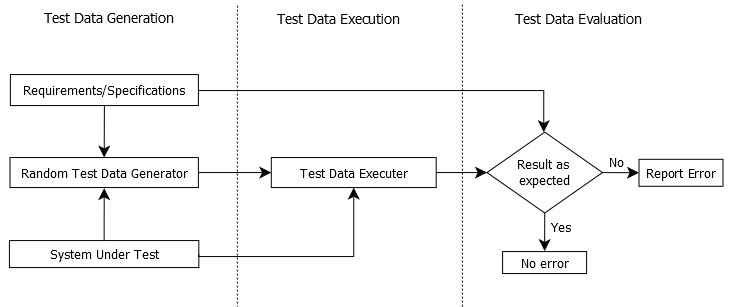
\includegraphics[width=14cm, height=6cm ]{chapter1/SoftwareTesting1.png}
		\caption{Three main phases of random testing}
	\label{fig:SoftwareTesting1}
\end{figure}

\section{The Problems}
\noindent Exhaustive testing of software is not always possible and the problem of selecting a test data set, from a large/infinite domain is often confronted. Test data set, as a subset of the whole domain, is carefully selected for testing the given software. Adequate test data set is a crucial factor in any testing technique because it represents the whole domain for evaluating the structural and/or functional properties~\cite{howden1986, mccabe1983}. Miller and Maloney were the first who comprehensively described a systematic approach of test data set selection known as path coverage. They proposed that testers select the test data so that all paths of the SUT are executed at least once~\cite{Miller1963}. The implementation of the strategy resulted in higher standards of test quality and a large number of test strategies were developed afterwords including boundary value analysis and equivalence class.

\noindent Generating test data set manually is a time-consuming and laborious exercise~\cite{korel1990}; Therefore, automated test data set generation is always preferred. Data generators can be of different types i.e. Path-wise, Goal-Oriented, Intelligent or Random~\cite{wiki2013}. Random generator produces test data set randomly from the whole domain. Unlike other approaches random technique is simple, widely applicable, easy to implement, faster in computation, free from bias and costs minimum overhead~\cite{Ciupa2007}. According to Godefroid et al., ``Random testing is a simple and well-known technique which can be remarkably effective in discovering software bugs"~\cite{Godefroid2005}.

\noindent Despite the benefits of random testing, its simplistic and non-systematic nature exposes it to high criticism~\cite{white1987}. Myers et al.~\cite{Myers2011} mentioned it as, ``Probably the poorest methodology of all is random-input testing...". However, Ciupa et al. reported that the above stated statement is based on intuition and lacks any experimental evidence~\cite{Ciupa2008a}. The criticism motivated the researchers to look into various aspects of random testing for evaluation and possible improvement. Adaptive random testing (ART)~\cite{Chen2008}, Restricted Random Testing (RRT)~\cite{Chan2002}, Feedback Directed Random Testing (FDRT)~\cite{Pacheco2007}, Mirror Adaptive Random Testing (MART)~\cite{Chen2003} and Quasi Random Testing (QRT)~\cite{Chen2005} are a few of the enhanced random testing techniques reported in the literature.

\noindent Random testing is also considered weak in providing high code coverage~\cite{cohen1997, Offutt1996}. For example, in random testing when the conditional statement  ``{\it if (x == 25) then ... }"  is exposed to execution then there is only one chance, of the ``{\it then...}" part of the statement, to be executed out of $2^\text{32}$ available options. If {\it x} is an integer variable of 32 bit value~\cite{Godefroid2005}. 

Random testing is no exception when it comes to the complexity of understanding and evaluating test results. Modern testing techniques simplify results by truncating the lengthy log files and displaying only the fault revealing test cases in the form of unit tests. Further efforts are required to get the test results of random testing in more compact and user-friendly way. 


\section{Research Goals} \label{ResearchGoals}
\noindent The main goal of the research study is to develop new techniques for automated random testing with the aim to achieve the following objectives:

\begin{enumerate}
\item To develop a testing strategy with the capability to generate more fault-finding test data.

\item To develop a testing technique for finding faults, fault domains and presentation of results on a graphical chart within the specified lower and upper bound. 

\item To develop a testing framework with focus on increase in code coverage along with generation of more fault-finding test data. 

\end{enumerate}

\section{Contributions}
The main contributions of the thesis research are stated below: 

\subsection{Dirt Spot Sweeping Random Strategy}
%Development of a new enhanced and improved form of automated random testing: the Dirt Spot Sweeping Random (DSSR) strategy. This strategy is based on the assumption that faults and unique failures reside in contiguous blocks and stripes. The DSSR strategy starts as a regular random+ testing strategy � a random testing technique with preference for boundary values. When a failure is found, it increases the chances of using neighbouring values of the failure in subsequent tests, thus slowly sweeping values around the failures found in hope of finding failures of different kind in its vicinity.
%The DSSR strategy is implemented in the YETI random testing tool. It is evaluated against random (R) and random+ (R+) strategies by testing 60 classes (35,785 line of code) with one million ($10^\text{6}$) calls for each session, 30 times for each strategy. The results indicate that for 31 classes, all three strategies find the same unique failures. We analysed the 29 remaining classes using t-tests and found that for 7 classes DSSR is significantly better than both R+ and R, for 8 classes it performs similarly to R+ and is significantly better than R, and for 2 classes it performs similarly to random and is better than R+. In all other cases, DSSR, R+ and R do not perform significantly differently. Numerically, the DSSR strategy finds 43 more unique failures than R and 12 more unique failures than R+.

The fault-finding ability of the random testing technique decreases when the failures lie in contiguous locations across the input domain. To overcome the problem, a new automated technique: Dirt Spot Sweeping Random (DSSR) strategy was developed. It is based on the assumption that unique failures reside in contiguous blocks and stripes. When a failure is identified, the DSSR strategy selects neighbouring values for the subsequent tests. Resultantly, selected values sweep around the failure, leading to the discovery of new failures in the vicinity. Results presented in Chapter~\ref{chap:DSSR} indicated higher fault-finding ability of DSSR strategy as compared with Random (R) and Random+ (R+) strategies.

\subsection{Automated Discovery of Failure Domain}
The existing random strategies of software testing discover the faults in the SUT but lack the capability of locating the fault domains. In the current research study, a fully automated testing strategy named, ``Automated Discovery of Failure Domain (ADFD)" was developed with the ability to find the faults as well as the fault domains in a given SUT and provides visualization of the identified pass and fail domains in the form of a chart. The strategy is described, implemented in YETI, and practically illustrated by executing several programs of one and two dimensions in the Chapter~\ref{chap:ADFD}. The experimental results proved that ADFD strategy automatically performed identification of faults and fault domains along with graphical representation in the form of chart.

\subsection{Invariant Guided Random+ Strategy}
Another random test strategy named, ``Invariant guided Random+ Strategy (IGRS)" was developed in the current research study. IGRS is an extended form of Random+ strategy guided by software invariants. Invariants from the given SUT are collected by Daikon--- an automated invariant detector for reporting likely invariants and adding them to the SUT as assertions. The IGRS is implemented in YETI and generates values in compliance with the added assertions. Experimental results presented in Chapter~\ref{chap:IGRS} indicated improved features of IGR+S in terms of higher code coverage and identification of subtle errors that R, R+ and DSSR strategies were either unable to accomplish or required larger duration.  

%\section{Structure of the Thesis}
%
%The rest of the thesis is organized as follows: In Chapter 2, a thorough review of the relevant literature is given. It includes a brief introduction of software testing techniques followed by automated random testing tools. Chapter~\ref{chap:DSSR} describes Dirt Spot Sweeping Random (DSSR) strategy, which is based on sweeping of fault clusters in the input domain. Chapter~\ref{chap:ADFD} presents the newly developed Automated Discovery of Fault Domains  (ADFD) strategy, which focuses on dynamically finding the faults and domains along with their graphical representation. Chapter~\ref{chap:IGR+S} presents the new strategy Invariant Guided Random+ Strategy (IGR+S) developed with the focus on quick identification of faults and increase in code coverage with the help of assertions. Chapter 6 summarizes contributions of the thesis research, discusses the strength and weaknesses of the study, gives conclusion and suggests avenues for future work. Chapter 7 ?



\section{Structure of the Thesis}
The rest of the thesis is organized as follows:\\

\hangindent=\parindent
\hangafter=1
\noindent
\textbf{Chapter~\ref{chap:softwareTesting}} provides an overview of the software testing process its common techniques along with their purpose.\\


\hangindent=\parindent
\hangafter=1
\noindent
\textbf{Chapter~\ref{chap:randomTesting}} is a thorough review of the relevant literature, describing random testing, various versions of random testing and the most commonly used automated testing tools based on random algorithms.\\

\hangindent=\parindent
\hangafter=1
\noindent
\textbf{Chapter~\ref{chap:DSSR}} describes newly proposed more efficient random testing technique known as Dirt Spot Sweeping Random (DSSR) strategy, which is based on sweeping of fault clusters in the input domain. The experimental study confirms that DSSR strategy is significantly better than R and R+ strategies. Finally the benefits and drawbacks of the DSSR strategy are discussed.\\

\hangindent=\parindent
\hangafter=1
\noindent
\textbf{Chapter~\ref{chap:ADFD}} presents the newly developed Automated Discovery of Fault Domains  (ADFD) strategy, which focuses on dynamically finding the faults and domains along with their graphical representation. It is shown that the presence of fault domains across the input domain, which have not been so far identified, can in fact be identified and graphically represented using 
ADFD strategy.\\

 
\hangindent=\parindent
\hangafter=1
\noindent
\textbf{Chapter~\ref{chap:IGRS}} presents the newly developed Invariant Guided Random+ Strategy (IGRS) developed with the focus on quick identification of faults and increase in code coverage with the help of assertions. It uses Daikon, a tool to generate likely invariants, to identify and incorporate invariants in the SUT code which serves as contracts to filter any vague test cases. \\

\hangindent=\parindent
\hangafter=1
\noindent
\textbf{Chapter~\ref{chap:conclusion}} is the concluding chapter, summarising the achievements of this research and discussing the future work.\\

 \hangindent=\parindent
 \hangafter=1
 \noindent
 \textbf{Appendix~\ref{chap:appendix1}} XXXXXXXX.\\




%Today, the primary focus of software companies is to achieve high quality. These companies spend an estimated thirty to ninety percent of the total software development cost on testing \ref{Beizer1990}, \ref{Standards2002}. In spite of spending 

%Software testing is the process of executing a software with specific test data followed by evaluation of the results to check whether it is working according to its specification or not \ref{Sommerville2006}.
% check here if we can replace specification with oracle or not.
%The test passes if the output complies to its specification and fails otherwise. The success of testing correlates with the number of failures found in the Software Under Test (SUT): a test is more successful if it finds more faults.

%It is interesting that program testing is used to show the presence of bugs, rather than absence of bugs [6]. Therefore the SUT that passes all the tests without returning a single failure does not guarantee that there is no fault. The testing process increases however the reliability and confidence of both the developers and the users in the tested product [7] [8] [9].

%Random testing is a black-box testing technique in which the SUT is executed against ran- domly selected test data. Test results obtained are compared either against the oracle defined, using SUT specifications in the form of assertions or exceptions defined by the programming language. The rapid increase in software development in today?s modern world prompts the need for automated testing to ensure high quality. The generation of random test data is com- paratively cheap and does not require too much intellectual and computation efforts [10] [11]. It is for this reason that various researchers have recommended this strategy for incorporation in automatic testing tools [12]. YETI [13] [14], AutoTest [15] [16], QuickCheck [17], Randoop [18], JArtage [19] are a few of the most common tools based on random strategy.


%%% ----------------------------------------------------------------------


%%% Local Variables: 
%%% mode: latex
%%% TeX-master: "../thesis"
%%% End: 
